\chapter{Casi d'Uso}
\section*{Inizializzazione sistema}

\begin{figure}[ht]
  \centering
  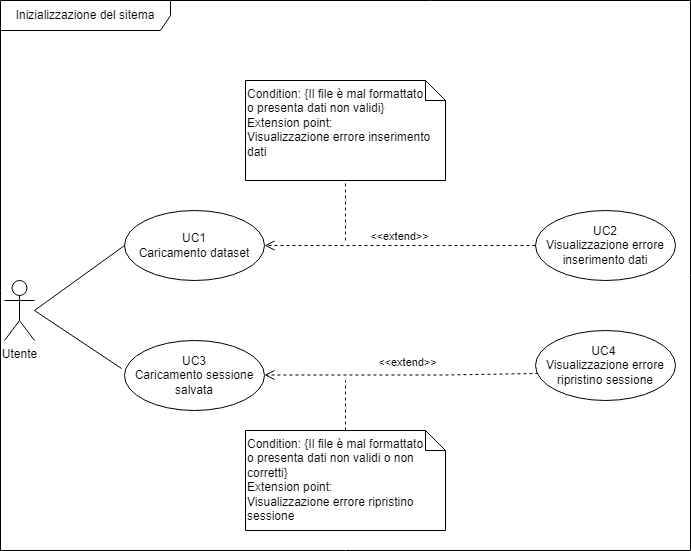
\includegraphics[width=\textwidth]{Iniz_sistema}
  \caption{Inizializzazione del sistema}
\end{figure}
\section{UC1 - Caricamento dataset}
\begin{itemize}
  \item \textbf{Descrizione:} l'utente vuole analizzare un nuovo dataset non presente nel sistema;
  \item \textbf{Attore primario:} utente;
  \item \textbf{Precondizioni:} il sistema è raggiungibile e funzionante. L’utente ha a disposizione un dataset in formato CSV;
  \item \textbf{Postcondizioni:} i dati presenti nel file vengono caricati nel sistema.
  \item \textbf{Scenario principale:}
  \begin{enumerate}
    \item L'utente accede al sistema;
    \item L'utente sceglie un file in formato CSV presente in locale e lo carica nel sistema;
    \item L'utente è pronto ad analizzare i dati.
  \end{enumerate}
  \item \textbf{Estensioni:} nel caso in cui il file sia in un formato non valido o i dati non siano validi:
    \begin{enumerate}
      \item Il caricamento non va a buon fine;
      \item Viene visualizzato un errore esplicativo [UC2].
    \end{enumerate}
\end{itemize}

\section{UC2 - Visualizzazione errore inserimento dati}
\begin{itemize}
  \item \textbf{Descrizione}: l'utente carica un file mal formattato o che presenta dati non validi, quindi visualizza un messaggio di errore esplicativo;
  \item \textbf{Attore Primario:} utente;
  \item \textbf{Precondizioni:} l’utente carica un file CSV contenente i dati da analizzare mal formattato o che presenta dati non validi;
  \item \textbf{Postcondizioni:} l'utente visualizza un messaggio di errore e i dati non vengono caricati;
  \item \textbf{Scenario Principale:}
  \begin{enumerate}
    \item L'utente visualizza un messaggio di errore esplicativo.
  \end{enumerate}
\end{itemize}

\section{UC3 - Caricamento sessione salvata}
\begin{itemize}
  \item \textbf{Descrizione:} l'utente vuole riprendere ad analizzare da dove si era interrotto o ha la necessità di visualizzare una sessione precedente;
  \item \textbf{Attore Primario:} utente;
  \item \textbf{Precondizioni:} l'utente che avvia l'applicativo ha salvato almeno una sessione di lavoro precedente;
  \item \textbf{Postcondizioni:} i dati di una sessione precedentemente salvata vengono ricaricati nel sistema;
  \item \textbf{Scenario Principale:}
  \begin{enumerate}
    \item L'utente accede al sistema;
    \item L'utente sceglie la sessione da caricare selezionando il file JSON desiderato tra quelli disponibili,
    cioè tra le sessioni salvate in precedenza;
    \item L'utente riprende da dove aveva salvato.
  \end{enumerate}
  \item \textbf{Estensioni:} nel caso in cui il file JSON selezionato non sia leggibile per qualche possibile errore di salvataggio:
    \begin{enumerate}
      \item Fallisce il caricamento della sessione precedente;
      \item Viene visualizzato un errore esplicativo [UC4].
    \end{enumerate}
\end{itemize}

\section{UC4 - Visualizzazione errore ripristino sessione}
\begin{itemize}
  \item \textbf{Descrizione}: l'utente carica un file mal formattato o che presenta dati non corretti, quindi visualizza un messaggio di errore esplicativo;
  \item \textbf{Attore Primario:} utente;
  \item \textbf{Precondizioni:} l’utente carica un file JSON contenente i dati da analizzare mal formattato o che presenta dati non validi o non corretti;
  \item \textbf{Postcondizioni:} l'utente visualizza un messaggio di errore e i dati non vengono caricati;
  \item \textbf{Scenario Principale:}
  \begin{enumerate}
    \item L'utente visualizza un messaggio di errore esplicativo.
  \end{enumerate}
\end{itemize}

\section{UC5 - Selezione tipo di grafico}
\begin{figure}[H]
 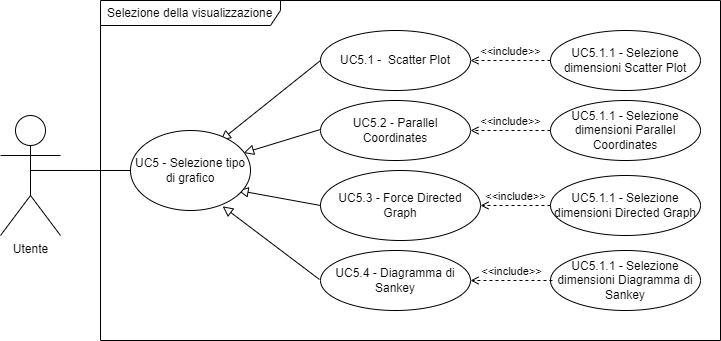
\includegraphics[width=\textwidth]{uc5.png}
 \caption{UC5 - Selezione tipo di grafico}
\end{figure}

 \begin{itemize}
     \item \textbf{Descrizione:} l'utente visualizza varie tipologie di grafico e ne sceglie una;
     \item \textbf{Attore primario:} utente;
     \item \textbf{Precondizioni:} il sistema è stato inizializzato [UC1];
     \item \textbf{Postcondizioni:} viene visualizzato il grafico desiderato;
     \item \textbf{Scenario principale:}
     \begin{enumerate}
       \item L'utente sceglie la visualizzazione desiderata tra quelle disponibili;
     \end{enumerate}
     \item \textbf{Generalizzazioni:} l'utente può selezionare una tra le possibili opzioni:
     \begin{enumerate}
         \item \textit{Scatter Plot} [UC5.1];
         \item \textit{Parallel Coordinates} [UC5.2];
         \item \textit{Force-Directed Graph} [UC5.3];
         \item \textit{Sankey Diagram} [UC5.4].
     \end{enumerate}
 \end{itemize}

\subsection{UC5.1 - Selezione Scatter Plot}
\begin{itemize}
    \item \textbf{Descrizione:} l'utente decide che visualizzazione di \textit{Scatter Plot} vuole vedere;
    \item \textbf{Attore primario:} utente;
    \item \textbf{Precondizioni:} il sistema è stato inizializzato [UC1];
    \item \textbf{Postcondizioni:} viene visualizzato il grafico \textit{Scatter Plot} selezionato;
    \item \textbf{Scenario principale:}
    \begin{enumerate}
      \item L'utente sceglie la visualizzazione desiderata tra quelle disponibili, decidendo tra varie visualizzazioni dello stesso grafico.
    \end{enumerate}
\end{itemize}

\subsection{UC5.2 - Selezione Parallel Coordinates}
\begin{itemize}
    \item \textbf{Descrizione:} l'utente decide che visualizzazione di \textit{Parallel Coordinates} vuole vedere;
    \item \textbf{Attore primario:} utente;
    \item \textbf{Precondizioni:} il sistema è stato inizializzato [UC1];
    \item \textbf{Postcondizioni:} viene visualizzato il grafico \textit{Parallel Coordinates} selezionato;
    \item \textbf{Scenario principale:}
    \begin{enumerate}
    \item L'utente sceglie la visualizzazione desiderata tra quelle disponibili, decidendo tra varie visualizzazioni dello stesso grafico.
    \end{enumerate}
\end{itemize}

\subsection{UC5.3 - Selezione Force-Directed Graph}
\begin{itemize}
    \item \textbf{Descrizione:} l'utente decide che visualizzazione di \textit{Force-Directed Graph} vuole vedere;
    \item \textbf{Attore primario:} utente;
    \item \textbf{Precondizioni:} il sistema è stato inizializzato [UC1];
    \item \textbf{Postcondizioni:} viene visualizzato il grafico \textit{Force-Directed Graph} selezionato;
    \item \textbf{Scenario principale:}
    \begin{enumerate}
      \item L'utente sceglie la visualizzazione desiderata tra quelle disponibili, decidendo tra varie visualizzazioni dello stesso grafico.
    \end{enumerate}
\end{itemize}

\subsection{UC5.4 - Selezione Sankey Diagram}
\begin{itemize}
    \item \textbf{Descrizione:} l'utente decide che visualizzazione di \textit{Sankey Diagram} vuole vedere;
    \item \textbf{Attore primario:} utente;
    \item \textbf{Precondizioni:} il sistema è stato inizializzato [UC1];
    \item \textbf{Postcondizioni:} viene visualizzato il grafico \textit{Sankey Diagram} selezionato;
    \item \textbf{Scenario principale:}
    \begin{enumerate}
      \item L'utente sceglie la visualizzazione desiderata tra quelle disponibili, decidendo tra varie visualizzazioni dello stesso grafico.
    \end{enumerate}
\end{itemize}


\section{UC6 - Filtri sui dati}
\begin{figure}[H]
  \centering
  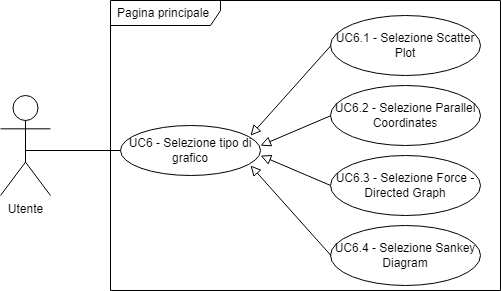
\includegraphics[width=\textwidth]{uc6.png}
  \caption{UC6 - Filtri sui dati}
\end{figure}

\begin{itemize}
  \item \textbf{Descrizione}: l'utente ha la possibilità di modificare la visualizzazione attraverso l'applicazione di filtri sui dati;
  \item \textbf{Attore primario}: utente;
  \item \textbf{Precondizioni}: l'utente ha selezionato la tipologia di grafico [UC5] e l'applicativo lo ha generato;
  \item \textbf{Postcondizioni}: i filtri applicati consentono di mostrare la nuova visualizzazione dei dati sul grafico;
  \item \textbf{Scenario principale}:
    \begin{enumerate}
      \item L'utente può impostare i filtri tramite una sezione dedicata;
      \item Il grafico mostra solo i dati con le caratteristiche corrispondenti alla scelta dei filtri.
    \end{enumerate}
\end{itemize}

\subsection{UC6.1 - Filtraggio per ID}
\begin{itemize}
  \item \textbf{Descrizione}: l'utente ha la possibilità di filtrare i dati in base ad un determinato ID;
  \item \textbf{Attore primario}: utente;
  \item \textbf{Precondizioni}: l'utente ha selezionato la tipologia di grafico [UC5] e l'applicativo lo ha generato;
  \item \textbf{Postcondizioni}: i dati visualizzati sono filtrati in base ad un determinato ID;
  \item \textbf{Scenario principale}:
    \begin{enumerate}
      \item L'utente inserisce l'ID desiderato;
      \item Il grafico mostra solo i dati con l'ID corrispondente.
    \end{enumerate}
\end{itemize}

\subsection{UC6.2 - Filtraggio per IP}
\begin{itemize}
  \item \textbf{Descrizione}: l'utente ha la possibilità di filtrare i dati in base ad un determinato IP;
  \item \textbf{Attore primario}: utente;
  \item \textbf{Precondizioni}: l'utente ha selezionato la tipologia di grafico [UC5] e l'applicativo lo ha generato;
  \item \textbf{Postcondizioni}: i dati visualizzati sono filtrati in base ad un determinato IP;
  \item \textbf{Scenario principale}:
    \begin{enumerate}
      \item L'utente inserisce l'IP desiderato;
      \item Il grafico mostra solo i dati con l'IP corrispondente.
    \end{enumerate}
\end{itemize}

\subsection{UC6.3 - Filtraggio per utente}
\begin{itemize}
  \item \textbf{Descrizione}: l'utente ha la possibilità di filtrare i dati in base ad un determinato utente;
  \item \textbf{Attore primario}: utente;
  \item \textbf{Precondizioni}: l'utente ha selezionato la tipologia di grafico [UC5] e l'applicativo lo ha generato;
  \item \textbf{Postcondizioni}: i dati visualizzati sono filtrati in base ad un determinato utente;
  \item \textbf{Scenario principale}:
    \begin{enumerate}
      \item L'utente inserisce il numero dell'utente desiderato;
      \item Il grafico mostra solo i dati con il numero dell'utente corrispondente.
    \end{enumerate}
\end{itemize}

\subsection{UC6.4 - Filtraggio per tipo evento}
\begin{itemize}
  \item \textbf{Descrizione}: l'utente ha la possibilità di filtrare i dati in base ad un determinato tipo di evento;
  \item \textbf{Attore primario}: utente;
  \item \textbf{Precondizioni}: l'utente ha selezionato la tipologia di grafico [UC5] e l'applicativo lo ha generato;
  \item \textbf{Postcondizioni}: i dati visualizzati sono filtrati in base ad un determinato tipo di evento;
  \item \textbf{Scenario principale}:
    \begin{enumerate}
      \item L'utente inserisce il tipo di evento desiderato;
      \item Il grafico mostra solo i dati con il tipo di evento corrispondente.
    \end{enumerate}
\end{itemize}

\subsection{UC6.5 - Filtraggio per data}
\begin{itemize}
  \item \textbf{Descrizione}: l'utente ha la possibilità di filtrare i dati in base alla data;
  \item \textbf{Attore primario}: utente;
  \item \textbf{Precondizioni}: l'utente ha selezionato la tipologia di grafico [UC5] e l'applicativo lo ha generato;
  \item \textbf{Postcondizioni}: i dati visualizzati sono filtrati in base alla data;
  \item \textbf{Scenario principale}:
    \begin{enumerate}
      \item L'utente inserisce il periodo temporale desiderato;
      \item Il grafico mostra solo i dati interni al periodo temporale corrispondente.
    \end{enumerate}
\end{itemize}

\subsection{UC6.6 - Filtraggio per applicazione}
\begin{itemize}
  \item \textbf{Descrizione}: l'utente ha la possibilità di filtrare i dati in base ad una determinata applicazione;
  \item \textbf{Attore primario}: utente;
  \item \textbf{Precondizioni}: l'utente ha selezionato la tipologia di grafico [UC5] e l'applicativo lo ha generato;
  \item \textbf{Postcondizioni}: i dati visualizzati sono filtrati in base ad una determinata applicazione;
  \item \textbf{Scenario principale}:
    \begin{enumerate}
      \item L'utente inserisce l'applicazione desiderata;
      \item Il grafico mostra solo i dati relativi all'applicazione corrispondente.
    \end{enumerate}
\end{itemize}


\section{UC7 - Accesso al manuale utente}
\begin{itemize}
  \item \textbf{Descrizione}: l'utente che ha un dubbio o vuole più informazioni sull'utilizzo dell'applicazione, deve avere accesso rapido al manuale utente;
  \item \textbf{Attore primario}: utente;
  \item \textbf{Precondizioni}: nessuna, l'opzione di accesso ai manuali deve essere sempre disponibile all'utente;
  \item \textbf{Postcondizioni}: viene visualizzato il manuale utente;
  \item \textbf{Scenario principale}:
  \begin{enumerate}
    \item L'utente seleziona il manuale utente;
    \item Viene visualizzato il manuale utente.
  \end{enumerate}
\end{itemize}

\section{UC8 - Salvataggio sessione}
\begin{itemize}
  \item \textbf{Descrizione:} l'utente salva la sessione di lavoro;
  \item \textbf{Attore primario:} utente;
  \item \textbf{Precondizioni:} l'utente ha svolto una sessione di lavoro sull'applicazione, in particolare potrebbe aver scelto un grafico specifico e modificato i parametri personalizzando la visualizzazione;
  \item \textbf{Postcondizioni:} l'utente possiede un file JSON in grado di recuperare grafico e parametri impostati durante la sessione di lavoro;
  \item \textbf{Scenario principale:}
  \begin{enumerate}
    \item L'utente sta lavorando sull'applicazione;
    \item L'utente seleziona la funzionalità ``Salvataggio sessione'';
    \item L'utente salva la sessione corrente.
  \end{enumerate}
\end{itemize}
